\chapter{Theoretische Grundlagen}
%NOTES:
%-> verteilte systeme zeug
 %   -> sync and async data exchange
  %  -> verschlüsselung
   % -> Authentifizierung
 %   -> Business Data Objects (BDO)
%    -> 
%websockets
%opcua
%knoten und kanten
%datenbanken
%was ist eine db?
%-> normalformen
%-> referenzielle integrität
%-> sql
%webdevelopment
%-> js frameworks
%-> vue
%-> JSON
%-> XML
%-> REST
%interfaces
%->general
%->impl. in JS
%->impl. in C++
%\section{SCADA}
%\section{Verteilte Systeme}
%\subsection{Synchrones Datenmodell}
%\subsection{Asynchrones Datenmodell}
\section{Security}
\subsection{Authentifizierung}
\subsection{Verschlüsselung}
\section{Safety}
\section{Websocket}
\section{Datenbanken}
Der Zweck eines Datenbanksystems ist es Daten persistent zu speichern und zur verfügung zu stellen.
Ein Datenbanksystem setzt sich aus einer Datenbasis, sowie einem\\ \ac{dbms} zusammen.
Dabei stellt die Datenbasis den Speicher der Datenbank dar und das \ac{dbms}, 
das Programm durch das der Zugriff auf die Datenbasis geschieht.
Das \ac{dbms} ist notwendig, um konkurierende Zugriffe auf die Datenbasis, von mehreren Nutzern zu Verwalten. \citep{Schubert:2007:3}
Meistens bietet das \ac{dbms} als Interface eine Netzwerkschnittstelle an (Server-Client Architektur), es gibt allerdings auch Datenbanken deren \ac{dbms} Teil der Applikation werden (z.B. SQLite).
\subsection{Relationale Datenbank}\label{subsec:relDB}
Im Falle einer relationalen Datenbank werden Daten in Form von Relationen abgespeichert.
Tabellen sind eine Darstellung von Relationen.\\
Jede Relation hat Attribute mit einem in der Relation einzigartigem Attributnamen.
Die Domaine eines Attributs ist die Menge aller Werte die ein Attribut annehmen kann.
Ist der Wert eines Attributs unbekannt oder noch nicht bestimmt, ist der Wert des Attributs \glqq{}NULL''.\citep{Studer:2016:2}
Werden Daten nun in einer Datenbank gespeichert, wird ein Wertetupel in eine Relation eingefügt.
Die Relationen sind nur das strukturelle theoretische Konzept, das sich hinter einer Relationenalen Datenbank verbirgt.
Anfangs dieses Abschnitts wurde gesagt dass Relationenn in Form einer Tabelle darstellbar sind.
Wenn den Relationen nun zur Ihrer Definition Wertetabellen zu Grunde liegen, 
ist es möglich zur Vereinfachung statt von Relationen, von Tabellen zu sprechen.
Das \ac{dbms} stellt eine Schnittstelle bereit um dem Nutzer die Daten zugänglich (\ac{crud} Operationen) zu machen.
Die Schnittstelle unterstützt meist die Sprache \ac{sql}. Diese Sprache ist in Abschnitt \ref{subsec:sql} genauer beschrieben.
Relationen können nicht nur als Tabelle ausgegeben werden, es ist auch möglich sie zu Verknüpfen.
Wenn keine Regel angegeben wird wie zwei Relationen Verknüpft werden sollen, wird das informatische Kreuzprodukt gebildet.
Das Bedeutet, dass jedes Wertetuple aus Relation A, mit jedem Wertetupel aus Relation B verknüft wird. 
Dadurch entsteht eine neue Realation.
In einer Datenbank existieren immer Schlüssel (Keys) innerhalb einer Tabelle.
Dabei gibt es drei Typen:
\begin{itemize}
  \item Primary-Key (Primärschlüssel)
  \item Unique-Key
  \item Foreign-Key (Fremdschlüssel)
\end{itemize}
Der Primary-Key muss als einzigster Schlüssel zwingend vorhanden sein. Er bestimmt nach was das \ac{dbms} die Datensätze ablegt.
Desshalb muss der Wert des Attributes das den Krimary-Key bildet innerhalb einer Tabelle einzigartig sein.
Das heist es darf maximal ein Wertetupel innerhalb einer Relation existieren, mit dem selben Wert des Primärschlüssels.
Der Primärschlüssel darf auch nicht \glqq{}NULL'' sein.
Ein Unique-Key stellt ein zusätzlichen Schlüssel dar, über die jeder Eintrag in eine Tabell eindeutig identifizierbar ist.
Wie auch der Primärschlüssel, darf dieser Schlüssel nicht \glqq{}NULL'' sein.
Er ist in jeder Tabelle nur optional vorhanden und kann auch mehrfach vorkommen.
Der Foreign-Key (Fremdschlüssel) ist ein Schlüssel der nur in einer relationalen \ac{dbms} existiert.
Er ermöglicht es, einen Verweises auf eine andere Tabelle zu definieren.
Zur Veranschaulichung sei folgendes Beispiel einer relationalen Datenstruktur,
auf einem \ac{sql} Server gegeben.
\begin{figure}[hbt]
  \centering
  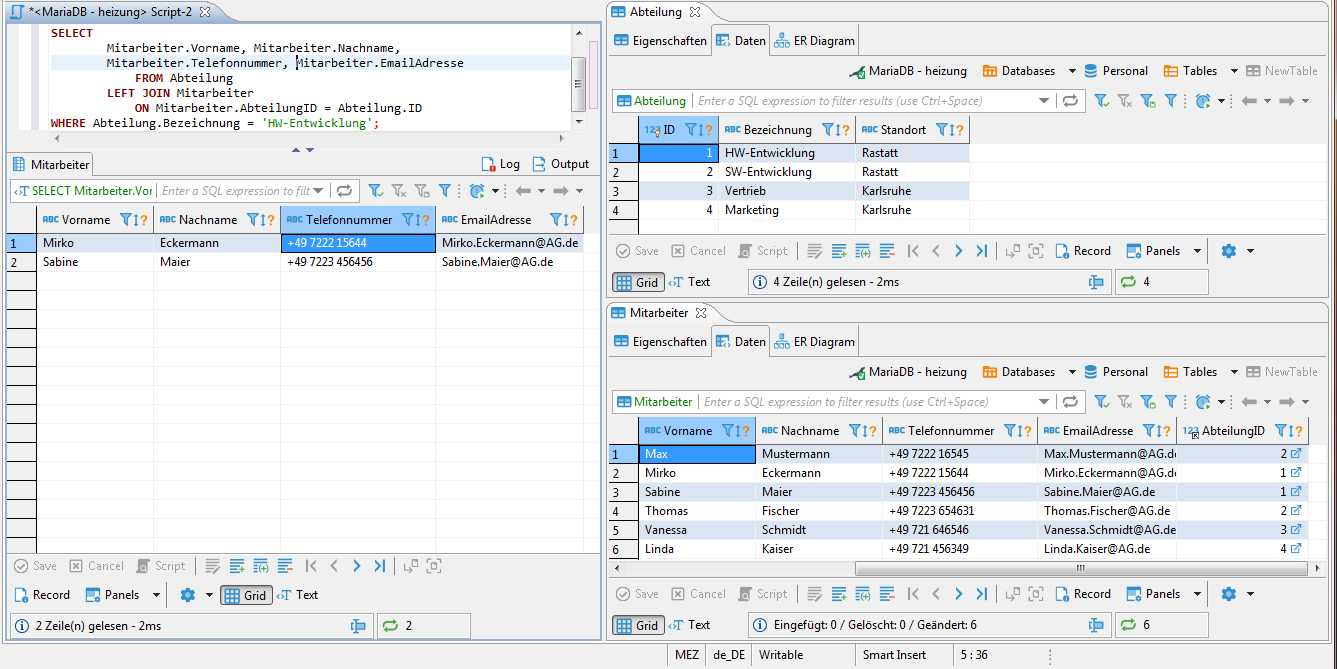
\includegraphics[width=\textwidth]{content/hauptteil/theoretischeGrundlagen/rec/exampleSQL.png}
\caption{Beispiel Datenstruktur}
 \label{fig:exampleSQLStructure}%%%%%%%%%%%%%AUSTAUSCHEN DURCH ERM!!!!!!!!!!!!!!!
\end{figure}
Wie in Abbildung \ref{fig:exampleSQLStructure} zu sehen, besteht die Datenbank \emph{Personal} aus zwei Tabellen.
Die erste Tabelle hat die Bezeichnung (\emph{Abteilung}) mit den Spalten \emph{ID}, \emph{Bezeichnung} sowie Standort.
Die Spalte \emph{ID} ist als primaryKey deklariert.
Die zweite Tabelle (\emph{Mitarbeiter}) enthält die Spalten 
\emph{Personalnummer}, \emph{Vorname}, \emph{Nachname}, \emph{Telefonnummer}, \emph{EmailAdresse}, \emph{AbteilungID}.
In dieser Tabelle ist die Personalnummer der Primärschlüssel.
Um eine Verknüpfung der Spalte \emph{AbteilungID} der Tabelle \emph{Mitarbeiter} zu der Tabelle \emph{Abteilung} herzustellen, 
wird ein Fremschlüssel definiert, der von der Spalte \emph{AbteilungID} der Tabelle \emph{Mitarbeiter} auf die Tabelle \emph{Abteilung}, 
unter Benutzung deren Primärschlüssels, verweist.
Die Benutzung eines solchen Frewmdschlüssels ist nicht zwingend notwendig um die Verknüfung nach dieser Regel zu ermöglichen,
Es ermöglicht aber die selbstständige Erhaltung der Datenbank der referenziellen Integrietät. 
Dabei hat man bei der Erstellung des Fremdschlüssels die Möglichkeit zu entschieden, was beim Löschen, oder beim Ändern, eines referenzierten Datensatzes geschehen soll.
Der Gängigste Umgang damit ist, dass man entweder das Löschen verbietet (\emph{on delete restrict},
oder das beim Löschen des referenzierten Datensatzes auf den referenzierenden Datensatz löscht (\emph{on delete cascade}).
Bei beiden Verfahren bleibt die referenzielle Integrietät erhalten, 
dass heist es gibt nach dem Löschen keine Referenzen die nicht aufgelöst werden können.

\subsection{\acs{sql}}\label{subsec:sql}
\acs{sql} ist eine Abkürzung für \acl{sql}. Dabei handelt es sich um eine Sprache, 
welche das Erzeugen und Verwalten von Datenstrukturen ermöglicht. 
Außerdem ermöglicht sie das Abfragen, Einfügen, Verändern, sowie Verknüpfen von Datensätzen.
Dabei unterscheidet sich \ac{sql} sehr von anderen Programmiersprachen.
So besteht der Ansatz bei \ac{sql} eher darin zu definieren, was man als Ergebnis möchte, 
sich aber um die konkrete Implementierung der Operation keinerlei Gedanken machen braucht.
Um dies zu demonstrieren ist das folgende Beispiel, auf Basis der Beispieldatenbank in Abbildung \ref{fig:exampleSQLStructure}, gegeben.
Nun möchte man alle Telefonnummern, Namen und E-Mail Adressen einer Abteilung haben, welche den Namen \emph{HW-Entwicklung} trägt.
Dazu ist es notwendig die Datensätze der Mitarbeitertabelle mit den Datensätzen der Abteilungstabelle, 
entsprechend des Fremsschlüssels in der Mitarbeiter Tabelle, zu kombinieren und alle Datensätze der so entstanden Tabelle auszugeben, 
welche die Abteilungsbezeichnung \emph{HW-Entwicklung} tragen. 
Die Query für diese Operation ist in Abbildung \ref{fig:exampleSQLQuery} abgebildet.
\begin{figure}[hbt]
  %\centering
  %\inputsql{content/hauptteil/theoretischeGrundlagen/rec/sqlQuery.sql}
  \inputminted{sql}{content/hauptteil/theoretischeGrundlagen/rec/sqlQuery.sql}
  \caption{Beispiel sqlQuery - Select mit Join}
  \label{fig:exampleSQLQuery}
\end{figure}
Die Antwort des Servers ist in Abbildung \ref{fig:exampleSQLStructure} unten links zu sehen.
Rechts seht man die Datensätze der beiden Quelltabellen des Queries.
Wahrscheinlich würde man diesen einfachen Datenbank Join, in C/C++, mit den Daten in Structures gespeichert, mittels verschachtelter For-Schleifen implementieren. Dass Problem bei dieser Implementierung ist, man muss durch jedes Element itterieren.
Die Datenbank hat zur Lösung dieses Problems bessere Algorithmen hinterlegt (Stichwort: binärer Suchbaum, Hash-Maps\dots).

\subsection{Stored Procedurs}\label{subsec:storedProc}
Ein \ac{sql} Server unterstützt nicht nur das Manipulieren und Ausgeben von Daten mit \ac{sql}, sondern auch das Speichern von Funktionen und Prozeduren.
Diese Prozeduren und Funktionen sind auch in \ac{sql} geschrieben.
Sie ermöglichen dem Entwickler das Auslagern komplexer \ac{sql} Querys.
Der wesentliche Unterschied zwischen einer Prozedur und einer Funktion besteht darin, dass eine Funktion einen Rückgabewert haben kann, eine Prozedur dagegen nicht.
Das Fehlen eines Rückgabewerts einer Prozedur stellt aber, entgegen der allgemeinen Erwartung, keine Einschränkung dar. 
Prozeduren und Funktionen akzeptieren auch sessionbezogene globale Variablen als \emph{OUT} Argument. 
Desweiteren haben Prozeduren entgegen Funktionen die Möglichkeit, SQL-Queries zur Laufzeit zusammenzusetzen und auszuführen.
Funktionenn können, in \ac{sql} Querys benutzt werden, Prozeduren nicht.
Prozesuren werden durch ein \emph{CALL} Befehl aufgerufen.


\section{OPC UA}
\ac{opcua} ist laut 
Der \ac{opcua} Standart ist in der IEC 62541 definiert.

\section{Echtzeit}
Laut Peter Scholz ist Echtzeit wie folgt definiert:\\
\glqq{}Unter Echtzeit versteht man den Betrieb
eines Rechensystems, bei dem Programme zur Verarbeitung
anfallender Daten ständig betriebsbereit sind, derart, dass die
Verarbeitungsergebnisse innerhalb einer vorgegebenen Zeitspanne
verfügbar sind. Die Daten können je nach Anwendungsfall nach
einer zeitlich zufälligen Verteilung oder zu vorherbestimmten
Zeitpunkten anfallen.''
\citep{Scholz:2005}\\
Das bedeutet, dass ein System nur dann echtzeitfähig ist wenn es die folgenden Bedingungen erfüllt:
\begin{itemize}
  \item Jede Komponente des Systems die an dem Prozess beteiligt ist, muss selbst echtzeitfähig sein.
  \item Die Rechenzeit der verwendeten Algorithmen muss endlich sein.
  \item Die verwendenten Transportprotokolle um dem Prozess Daten zuzuführen bzw. Daten zu entnehmen müssen die Echtzeitfähigkeit unterstützen.
\end{itemize}
Wenn die obere Definion nun auf das Ethernet oder das \ac{tcp} Protokoll angewand wird, fällt schnell auf, 
dass diese beide normalerweise nicht echtzeitfähig sind.
Ethernet verhindert auf dem BUS (physikalischer Layer) keine Kollistionen sondern erkennt diese nur. 
Wenn eine Kollision erkannt wurde, 
wird das Senden auf den BUS abgebrochen und nach einer zufälligen Zeit erneut versucht.
Dieses Verfahren nennt nennt man \ac{CSMA/CD}. 
Wer den Zugriff auf den Bus bekommt ist Zufall.
Deshalb ist nicht garatiert, dass man innerhalb einer definierten Zeitspanne, die Daten übertragen kann.
Man kann dieses Problem allerdings umgehen indem man im physikalischen Layer bereits dafür sorgt, 
dass keine Datenkollision auftreten kann. Dies ist zum Beispiel durch den Einsatz von Switches möglich.
Diese trennen die einzelnen Sender voneinander und verhindern damit gezielt Kollisionen.
Man muss anmerken man immernoch nicht vollständig Echtzeitfähig Daten übertragen kann, 
denn das Netzwerk muss auch auf die aufkommende Datenlast ausgelegt sein.
Dadurch ist es möglich mit Ethernet in einer kontrollierten Umgebung Daten in Echtzeit zu übertragen.
Ein weitverbreiteter Irrtum ist, dass Echtzeitfähigkeit bedeutet etwas müsse besonders schnell reagieren, 
es genügt dass die Zeit definiert und endlich ist.